 \chapter{EOM Combs}

In this chapter, I discuss the generation of high-repetition-rate frequency combs through electro-optic modulation of a continuous-wave laser – so-called EOM combs \cite{Metcalf2013}\color{red}OTHERS\color{black}. This scheme represents an alternative to parametric generation of HRR combs in Kerr resonators, and as the technology matures it will likely find a niche in the application space that leverages its long-term stability, lack of moving parts, and possibility for robust turn-key operation. First I present the operational principle and experimental results that represent the first generation of a coherent octave-spanning supercontinuum and detection of an active-modulation-based frequency comb’s carrier-envelope offset frequency without an external optical reference. Then I provide a detailed discussion of the noise properties of the EOM comb, and I conclude with a proposal for future work.

\section{Principle of operation}
Generally, the EOM comb concept consists of passing a CW laser through cascaded phase and intensity modulators to generate a train of chirped pulses, and then propagating this pulse train through a dispersive medium to temporally compress the pulses to near their bandwidth-limited pulse duration. In a typical implementation, the pulses are generated with normal (in contrast with anomalous) chirp – the carrier frequency increases over the pulse duration. This allows compression via propagation in standard, anomalously dispersive optical fiber. In this case an expression for the electric field before temporal compression results from the product of the field $E_oe^{-i\omega_ct}$ with the intensity modulation $\frac{1}{2}\left\{\mathrm{exp}\left[i\frac{\pi}{4}(1+\sin{\omega_rt})\right]+\mathrm{exp}\left[-i\frac{\pi}{4}(1+\sin{\omega_rt})\right]\right\}$ and the phase modulation $\mathrm{exp}\left[i\beta_m \sin{\omega_r t}\right]$. Here representing the intensity modulation as the sum of exponential terms (instead of using the equivalent representation with $\cos{\omega_rt}$) is indicative of the fact  that the intensity modulation arises from simultaneous phase modulation in two paths. The resulting electric field (up to a constant overall phase shift relative to the previous expressions) is:
\begin{equation}
E=E_o\cos\left(\frac{\pi}{2}\sin^2{\frac{\omega_rt}{2}}\right)e^{i\omega_ct-i\beta_m\cos{\omega_rt}}.
\end{equation}
This can be understood as the product of a time-varying real amplitude $a(t)=E_o\cos\left(\frac{\pi}{2}\sin^2{\frac{\omega_rt}{2}}\right)$ and a phase factor from which the instantaneous carrier frequency $\omega(t)=\omega_c+\omega_r\beta_m\sin{\omega_rt}$ can be calculated. The carrier frequency $\omega(t)$ is increasing when the amplitude $a(t)$ is at its maximum, corresponding to normal chirp on the pulses.

\section{Detection of the carrier-envelope offset frequency of an EOM comb}

Here I describe generation of an EOM comb with 10 GHz repetition rate and subsequent measurement of its carrier-envelope offset frequency. The experimental setup is depicted in Fig. 1a. The basic experimental scheme consists of the following steps: 1. Initial generation and temporal compression of the EOM comb pulse train; 2. Spectral broadening and temporal re-compression; 3. Noise reduction using a Fabry-Perot filter cavity; and 4. Octave-spanning supercontinuum generation and detection of the carrier-envelope offset frequency. The results described below represent the first time a frequency comb based on active modulation of a CW laser has been self-referenced. Key to the success of this approach is the implementation of nonlinear spectral broadening in two stages, which allows the second stage to be seeded with $\sim$100 fs pulses for coherent supercontinuum generation, and also the noise reduction stage, described below. 

To generate the initial train of chirped pulses, a telecom-band continuous-wave laser is passed through cascaded phase and intensity modulators driven with a 10 GHz microwave signal. The intensity modulator is biased at the 50 \% transmission point and driven with an RF amplitude of $V_\pi/2$.   The phase modulator is driven with modulation depth of $\sim31\pi/4\sim24.3$ rad. The relative phase between the modulators is set such that the phase applied by the phase modulator is at a minimum when the transmission of the intensity modulator is highest; this yields a train of up-chirped pulses. Simulated temporal intensity and instantaneous carrier-frequency profiles are shown in Fig. 1b, and a simulated optical spectrum is overlaid on an experimental measurement in Fig. 1c.

 % % % % % PulsePickedTrains]
\begin{figure}[htpb]
	\begin{center}
		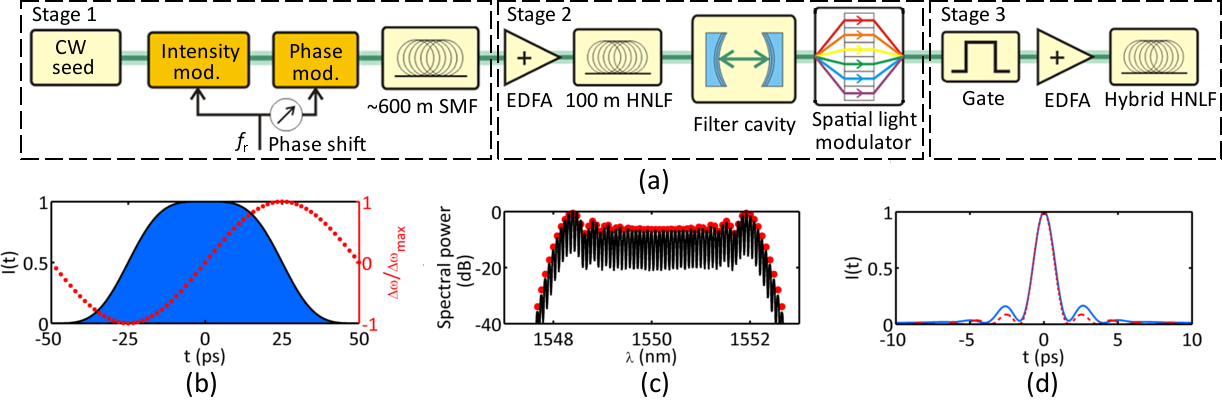
\includegraphics[width=15cm]{\FigPath/Figures/EOMCombs/EOMCSchematic.png}
	\end{center}
	\caption[Figure Title]{\textbf{BFCaption.} Caption}
	\label{fig:PPConcept}
\end{figure} 


Next, the chirped pulse train is propagated through 600 m of anomalously-dispersive SMF. The length of SMF that is appropriate for pulse compression depends on the bandwidth of the optical pulses to be compressed; equivalently it depends on both the phase-modulation depth and the repetition rate of the pulse train. This temporal compression reduces the duration of the optical pulses from $\sim$50 ps to $\sim$ 1.5 ps. A simulation of the resulting intensity profile is presented in Fig. 1d. 

The compressed pulses are amplified to 400 mW average power in an erbium-doped fiber amplifier and launched into 100 m of HNLF. This section of HNLF has chromatic dispersion that is small and normal; this is carefully chosen to chirp the pulses via self-phase modulation while avoiding soliton-fission dynamics. The result is a train of chirped $\sim$1.5 ps pulses exiting the fiber.  In Fig. 2a we present the measured optical spectrum of this pulse train, as well as results of a numerical simulation of the spectral broadening in the 100 m of normally-dispersive HNLF. These simulations are conducted using the nonlinear Schrodinger equation (NLSE) including third order dispersion, taking as initial conditions the calculated intensity profile of the EOM comb pulses shown in Fig. 1d. The dispersion values for the HNLF used in the simulation are $D=-0.04$  ps/nm$\cdot$km and $D'=0.003$ ps/nm$^2\cdot$km, close to the values specified by the manufacturer. The simulation method is described in detail in App. \ref{NumericalSims}.

After propagation through the first section of HNLF, the pulses are passed through a high-finesse Fabry-Perot cavity for suppression of optical frequency fluctuations as discussed below. Then the pulses are temporally compressed again, this time using a spatial light modulator (SLM) \cite{Weiner2000}; narrow spectral regions are resolved using a grating and passed through individually controlled delaying elements, then recombined. The SLM applies 2\textsuperscript{nd}, 3\textsuperscript{rd}, and 4\textsuperscript{th} order chromatic dispersion, which simulations indicate is sufficient to compress the pulses to $\sim$130 fs, nearly the transform limit. This is shown in Fig. 2b. It would also be possible to compress the pulses via propagation in an appropriate length of SMF, although this is less convenient than the compression of the initial EOM comb pulse train in SMF described above due to stronger fluctuations in the output over time associated with the nonlinear origin of the chirp. Figs. 2b and 2c present the output intensity profile and the evolution of the intensity profile, respectively, in simulated compression in SMF. Because the pulses are broadband, temporally short, and reasonably high energy, these simulations are performed including the full dispersion profile of SMF and the Kerr nonlinearity.






The temporally compressed $\sim$130 fs pulses are then passed through a Mach-Zehnder modulator functioning as an electro-optic gate for repetition-rate downsampling (see Chapter \ref{PulsePicking}). The gate selectively transmits every fourth pulse, reducing the repetition rate of the pulse train to 2.5 GHz. This facilitates coherent supercontinuum generation in a second stage of spectral broadening by increasing the pulse energy that can be achieved at a given average power. Note that this step is convenient but not strictly necessary, as shown in Ref. \cite{Beha2017}. 

The downsampled 2.5 GHz pulse train is amplified to an average power of 1.4 W, resulting in a train of $\sim$ 0.56 nJ pulses. This pulse train is propagated through 8 m of hybrid HNLF, yielding the spectrum shown in Fig. 2d. This hybrid HNLF consists of two segments with different dispersion profiles, with each segment serving a different purpose. The first segment is 30 cm long and highly dispersive ($D=6$  ps/nm$\cdot$km), and generates a dispersive wave centered at 1090 nm. The second segment is 7.7 m long and has lower dispersion ($D=1.5$  ps/nm$\cdot$km), and generates a Raman-self-frequency-shifted soliton centered near 2150 nm. The effect of each of these fibers on the output spectrum can be understood by investigating propagation in each section separately. To do this we use the LaserFOAM program \cite{Amorim2009}, which employs the generalized NLSE including Raman scattering, self-steepening, and 2nd- through 4th-order dispersion. The simulations are run independently, and both take as their initial conditions 170 fs Gaussian pulses with 350 pJ energy, close to the energy coupled into the HNLF after accounting for losses. The results of these simulations are plotted in Fig. 2d. 

 % % % % % PulsePickedTrains]
\begin{figure}[htpb]
	\begin{center}
		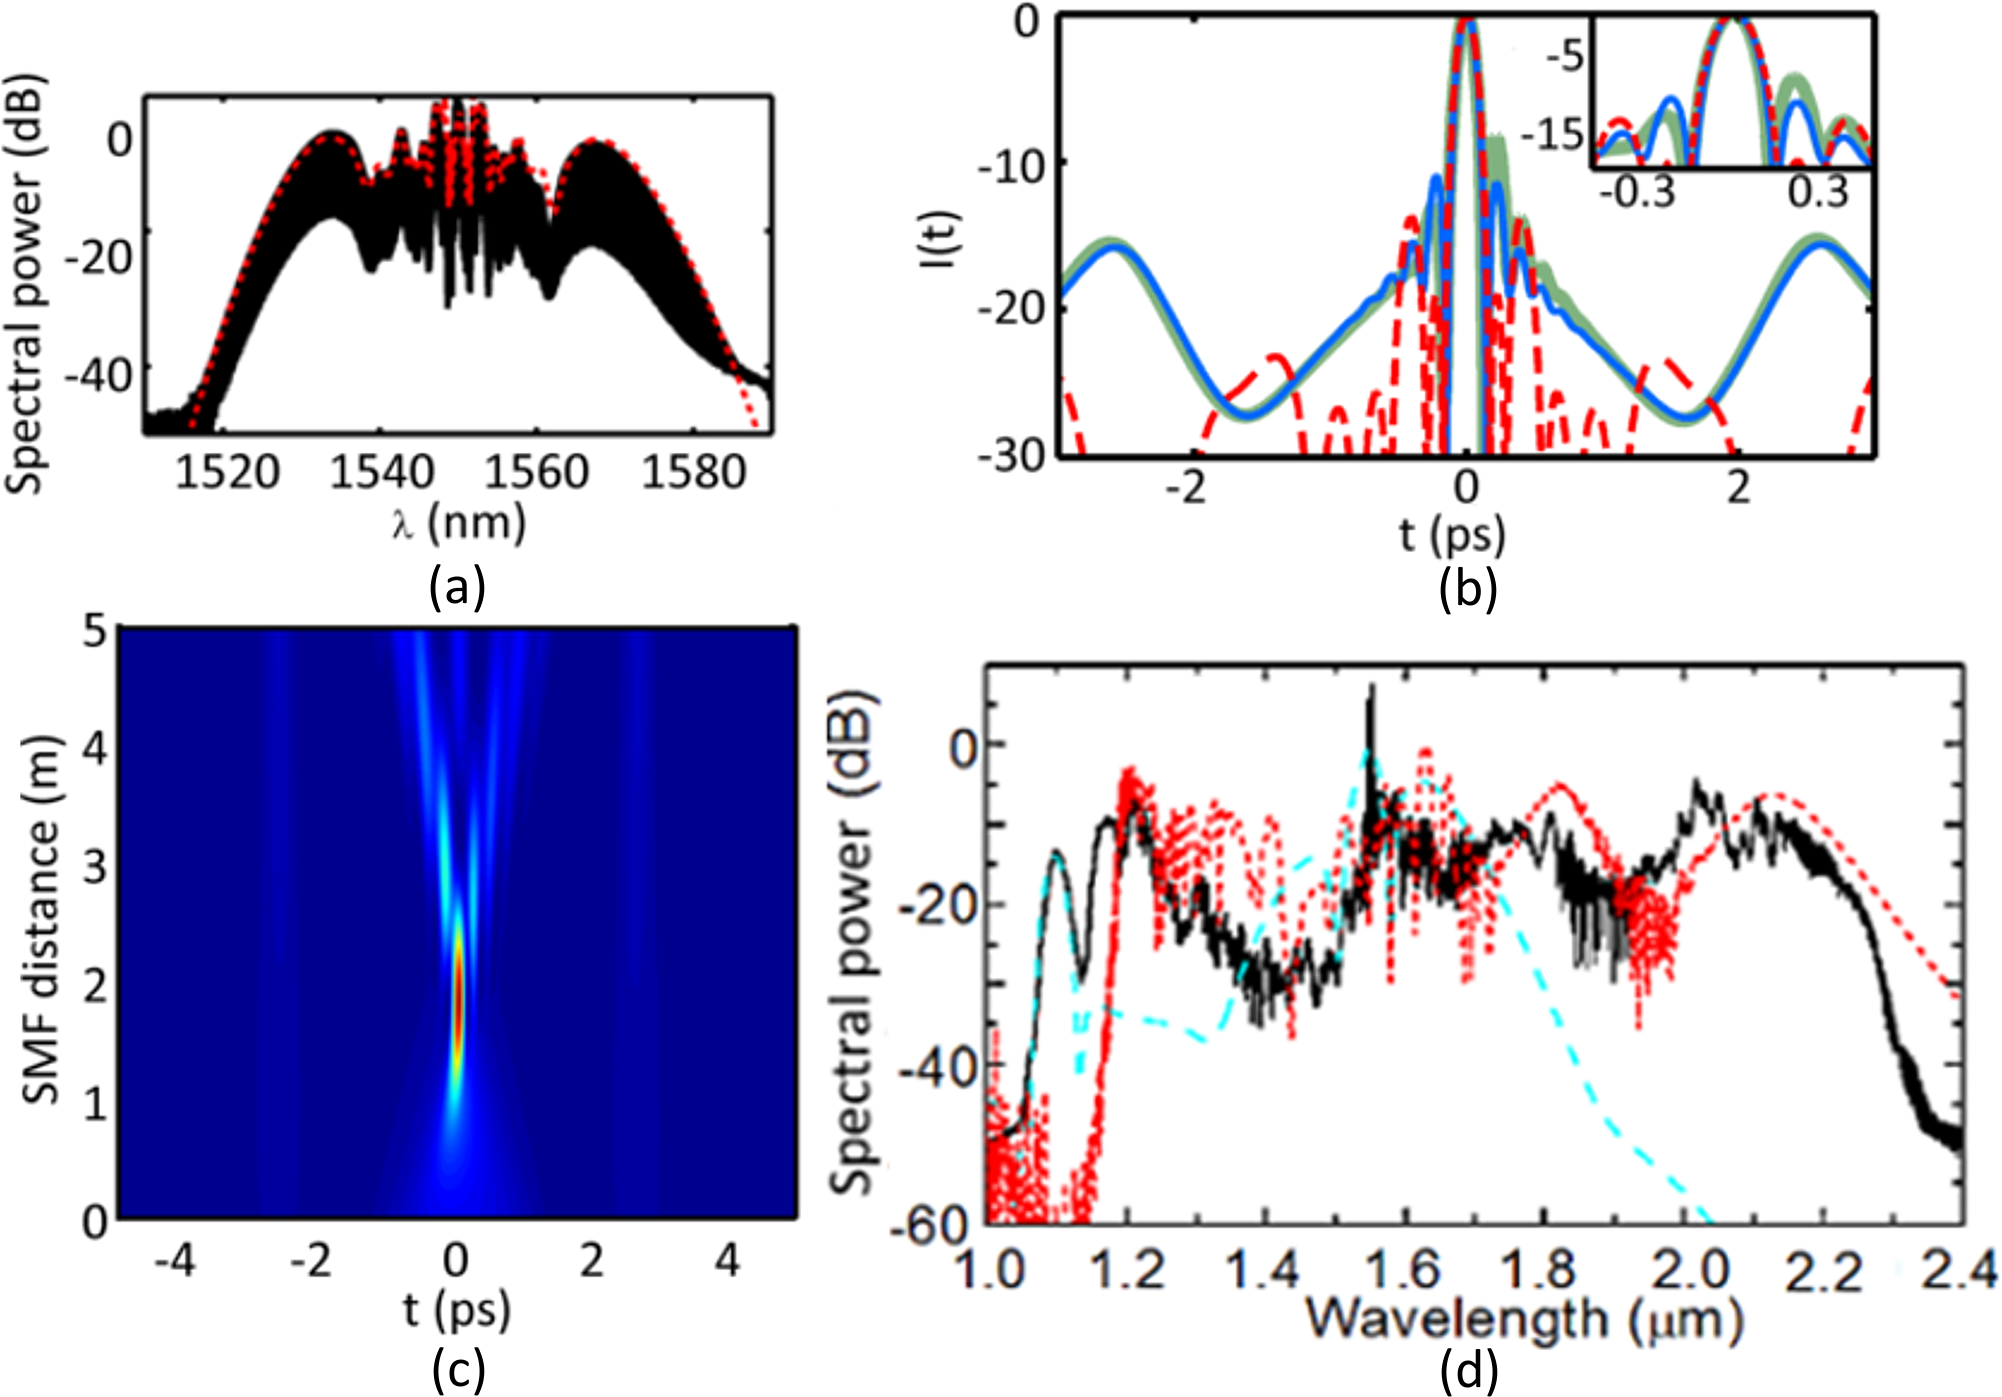
\includegraphics{\FigPath/Figures/EOMCombs/EOMC_spectraWsims.png}
	\end{center}
	\caption[Figure Title]{\textbf{BFCaption.} Caption}
	\label{fig:PPConcept}
\end{figure} 

The supercontinuum generated in the hybrid HNLF is coherent and suitable for $f-2f$ self-referencing. To detect the carrier-envelope offset frequency of the EOM comb, we pass the pulse train through an interferometer consisting of a dichroic mirror, a delay stage in one path, and a 10 mm sample of periodically-poled lithium niobate that generates the second harmonic of supercontinuum light at 2140 nm.  The dichroic mirror and delay stage enable adjustment of the relative timing between the native 1070 nm and doubled 2140 nm components of the supercontinuum so that they are temporally coincident. An optical band-pass filter centered at 1070 nm selects the supercontinuum components required for self-referencing, shown in Fig. 3a, and impinging the filtered light on a photodetector reveals the carrier-envelope offset frequency of the EOM comb, shown in Fig. 3b. Note that downsampling introduces an ambiguity in the offset frequency due to the increased density of comb modes in the downsampled pulse train; this ambiguity can be removed by measuring the change in measured offset frequency with a change in $f_r=\omega_m/2\pi$ provided by the synthesizer driving the modulators. 




\begin{figure}[htpb]
	\begin{center}
		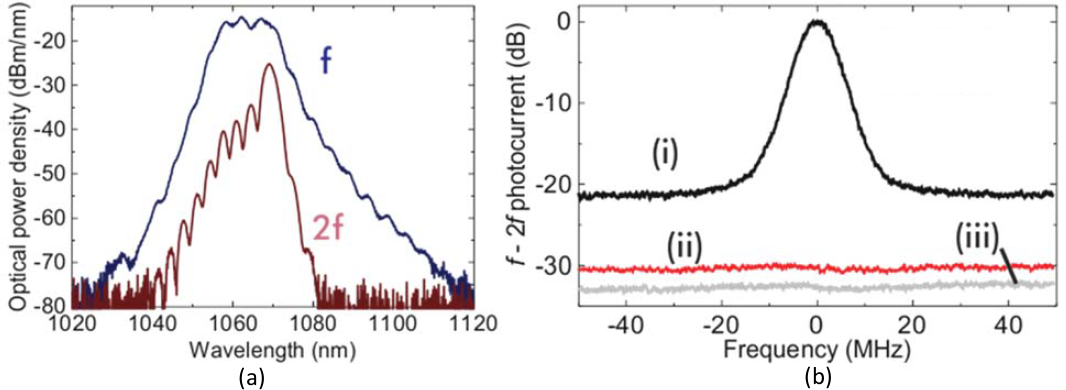
\includegraphics[width=15cm]{\FigPath/Figures/EOMCombs/EOMC_f0fromOptica.png}
	\end{center}
	\caption[Figure Title]{\textbf{BFCaption.} Caption}
	\label{fig:PPConcept}
\end{figure} 



\section{Noise in EOM Combs}

An important difference between the EOM comb scheme and other approaches for generation of frequency combs is that the repetition rate is derived directly from a microwave source and is directly multiplied by a factor $N$ to yield the optical frequency of mode number $N$ from the pump (where $N=0$). Therefore, the contribution to the optical frequency noise of mode number $N$ from the microwave source scales with the mode number $N$, and the contribution to the power spectrum of frequency noise scales as $N^2$. This presents a challenge in the generation of coherent supercontinuum light, where the modes relevant for $f-2f$ self-referencing are far separated from the pump laser. The factor by which the noise on the modulation tone $f_r$ is multiplied to determine its contribution to the noise on the measured carrier-envelope offset frequency is the ratio between the comb’s carrier frequency (the frequency of the seed laser) and the repetition rate: $N=f_c/f_r=$19340 for the 10 GHz comb discussed above (where $f_c=$193.4 THz for a 1550 nm pump laser). This contribution is shown in Fig. 3a, along with the contribution from the CW seed laser. The noise on $f_r$ results from technical noise on the synthesizer tone at low Fourier frequencies and approaches a white Johnson-Nyquist (thermal) phase-noise floor of -177 dBm/Hz at high Fourier frequencies. As discussed in Ref. \cite{Beha2017}, unmitigated multiplication of this noise floor by the factor $N=$19340 leads to a supercontinuum with optical frequency fluctuations that are large enough to prevent detection and measurement of $f_0$. 

To address this problem and enable $f-2f$ self-referencing of our comb, we pass the comb through a Fabry-Perot filter cavity whose free-spectral range is actively stabilized to the comb’s mode spacing. The filter cavity’s Lorentzian transfer function reduces the optical frequency fluctuations of the comb modes at high frequency – these fluctuations are averaged over the photon lifetime of the cavity. This enables generation of a supercontinuum with resolvable modes that is suitable for $f-2f$ self-referencing and measurement of $f_0$. 

The filter cavity used for this 10 GHz comb has a 7.5 MHz linewidth; equivalently, it has finesse of $F\sim$1333. The effect of passing the comb through the cavity is demonstrated concretely in Fig. 3b, where we compare the lineshape of a heterodyne beat between the supercontinuum and a CW laser with 1319 nm wavelength with and without the filter cavity in place. The signal-to-noise ratios for the beat with and without the filter cavity are 40 dB and 17 dB, respectively.


\begin{figure}[htpb]
	\begin{center}
		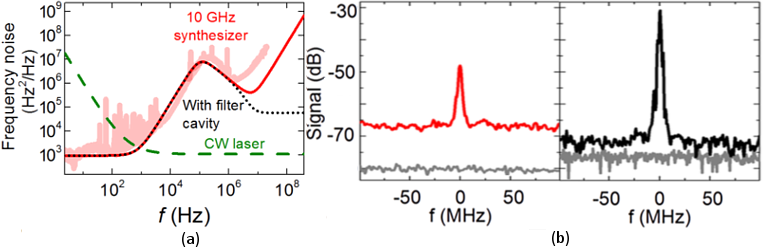
\includegraphics[width=15cm]{\FigPath/Figures/EOMCombs/EOMC_NoiseFigure_thesis.png}
	\end{center}
	\caption[Figure Title]{\textbf{BFCaption.} Caption}
	\label{fig:PPConcept}
\end{figure} 



\begin{figure}[htpb]
	\begin{center}
		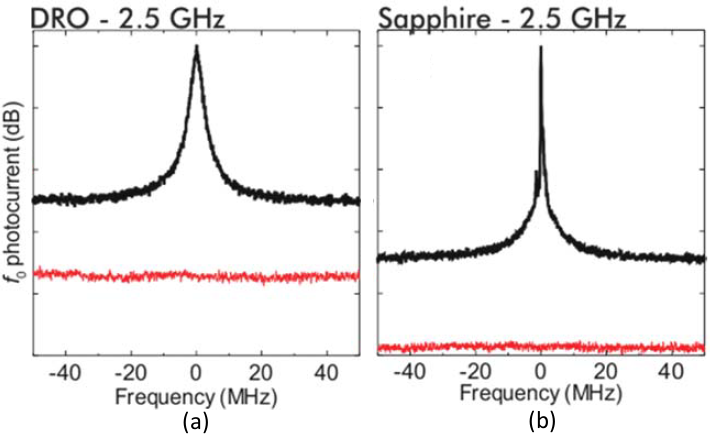
\includegraphics[width=10cm]{\FigPath/Figures/EOMCombs/EOMC_f0_diffosc_thesis.png}
	\end{center}
	\caption[Figure Title]{\textbf{BFCaption.} Caption}
	\label{fig:PPConcept}
\end{figure} 



